% ======================================================================
% MAT670 -- Lectures 7 and 8 (source: MAT670_78, pp. 1--31)
% First-pass transcription: "clean + fill gaps".
% ======================================================================

\chapter{Lecture 7: A short introduction to configuration spaces}
\label{L07:ch:lecture7}

\section{Configuration spaces}
\label{L07:sec:confspaces}

A \emph{configuration space} is a topological space that records the possible
configurations of an object we wish to study. For example:
\begin{itemize}
  \item the $2^N$ possible results of $N$ coin flips
    \added{(a discrete space $\{0,1\}^N$ with $2^N$ points)};
  \item the tilings of a checkerboard by dominoes \added{(again a finite set)};
  \item the positions and orientations of a polytope in space
    \added{(for a polytope with no symmetries this is $\R^3\times\SO(3)$; in general
    one divides $\SO(3)$ by the rotational symmetry group of the polytope)};
  \item the configurations of a mechanical linkage;
  \item the positions (and velocities) of particles in a box.
\end{itemize}

This last example is the one most closely related to what we want to study, and to the
first few lectures: positions of points in space.

\begin{definition}[Configuration space of $N$ points]
\label{L07:def:conf}
Let $X$ be a topological space. The \emph{(classical) configuration space of $N$
distinct labelled points in $X$} is
\[
  C^N(X) = \Conf(N,X) = \prod_{i=1}^N X \setminus \Delta,
  \qquad
  \Delta = \{(x_i)_{i=1}^N : x_i = x_j \text{ for some } i\neq j\},
\]
\added{with the subspace topology from the product $X^N$.}
\orig{crossed out: ``statistical mechanics'', ``also study''}
\end{definition}

\begin{exercise}
\label{L07:ex:weyl}
Think about how this might be related to the Weyl group associated to the root system
$A_n$.
\added{(Hint: take $X=\R$ and $N=n+1$. The Weyl group of $A_n$ is the symmetric group
$\Sigma_{n+1}$, acting on $\R^{n+1}$ by permuting coordinates, and its reflecting
hyperplanes are exactly the hyperplanes $x_i=x_j$ that make up $\Delta$. This is taken up
again in Section~\ref{L07:sec:weyl}.)}
\end{exercise}

There are also \emph{unlabelled} versions, $\Conf(N,X)/\Sigma_N$, where the symmetric
group $\Sigma_N$ acts by permuting the indices. When $X$ is endowed with a metric we can
also consider \emph{reduced} versions, $\Conf(N,X)/\operatorname{Isom}(X)$.
\added{(One can of course do both: $\Conf(N,X)/(\Sigma_N\times\operatorname{Isom}(X))$.)}
So the unlabelled version picks a single representative class for each permutation of the
indices, and the reduced version divides out by the symmetries of the ambient space.

\begin{example}[$\Conf(N,\R)$]
\label{L07:ex:confR}
We have $\Conf(N,\R)=\R^N\setminus\Delta$.
\begin{itemize}
  \item \emph{Unlabelled:} each point of $\Conf(N,\R)/\Sigma_N$ has exactly one
    representative with $x_1<x_2<x_3<\dots<x_N$, so we can choose to work in this region
    of the space.
    \added{$\R^N\setminus\Delta$ has $N!$ connected components, one for each ordering of
    the coordinates; each is an open convex cone, hence contractible, and $\Sigma_N$
    permutes them simply transitively.}
  \item \emph{Reduced:} we can shift one of the $x_i$ to $0$, for example the smallest.
    Together with the ordering this gives $\{0=x_1<x_2<\dots<x_N\}$.
    \added{(Modulo translations, the ordered region becomes the open cone
    $\{0<x_2<\dots<x_N\}\subset\R^{N-1}$; if reflections $x\mapsto -x$ are divided out as well, one may in addition
    fix the order of the two ``outer'' gaps.)}
\end{itemize}
\end{example}

\begin{center}
\begin{tikzpicture}[scale=0.9]
  % N = 2
  \fill[blue!8] (0,0) -- (2.4,2.4) -- (0,2.4) -- cycle;
  \draw[->] (-1.2,0) -- (2.6,0) node[right] {$x_1$};
  \draw[->] (0,-1.2) -- (0,2.6) node[above] {$x_2$};
  \draw[dashed] (-1.2,-1.2) -- (2.4,2.4) node[above right] {$\Delta$};
  \draw[very thick,addcol] (0,0.05) -- (0,2.4);
  \fill[white] (0,0) circle (2pt); \draw (0,0) circle (2pt);
  \node[align=center] at (0.7,1.75) {\small $x_1<x_2$};
  \node[addcol,left] at (0,1.2) {\small $x_1=0$};
\end{tikzpicture}
\end{center}
\noindent\textit{Figure:} $\Conf(2,\R)=\R^2\setminus\Delta$. The shaded half-plane
$\{x_1<x_2\}$ is a copy of the unlabelled space; the thick ray $\{0=x_1<x_2\}$ is the
reduced unlabelled space.
\orig{p.\,3 also sketches $N=3$, labelled ``$x_1=0$'', ``$x_1<x_2$'', ``$0<x_2<x_3$''}

\begin{example}[$\Conf(N,\Sph^2)$]
\label{L07:ex:confS2}
Consider labelled distinct points on a sphere. The reduced space is the space of $N$
labelled points on $\Sph^2$ modulo \emph{ambient} rotations.
For $N=4$: two configurations that differ by a rotation of the sphere are the same point of
the reduced space; a configuration and its mirror image are in general \emph{not} related by
a rotation, but they may become identified in the unlabelled space after relabelling
(e.g.\ swapping the labels $2$ and $3$).
\orig{p.\,4: sketches of 4 labelled points on spheres}
\added{(If one divides by all of $\operatorname{Isom}(\Sph^2)=\Orth(3)$ rather than by
$\SO(3)$, mirror images are identified as well.)}
\end{example}

\section{Braid groups}
\label{L07:sec:braid}

These spaces are related to the Artin braid groups, which we may define as follows.

\begin{definition}[Braid groups]
\label{L07:def:braid}
The \emph{braid group} and the \emph{pure braid group} of $X$ (on $N$ strands) are
\[
  B_N(X) = \pi_1\big(\Conf(N,X)/\Sigma_N\big),
  \qquad
  P_N(X) = \pi_1\big(\Conf(N,X)\big).
\]
\added{For $X=\R^2$ these are Artin's braid group $B_N$ and pure braid group $P_N$.
Since $\Conf(N,X)\to\Conf(N,X)/\Sigma_N$ is a covering map with deck group $\Sigma_N$, for
connected $\Conf(N,X)$ there is a short exact sequence
$1\to P_N(X)\to B_N(X)\to\Sigma_N\to 1$.}
\end{definition}

To see why these are called braid groups, consider what a path is in $\Conf(N,\R^2)$.
Fix a base point $x_0=(x_0^1,\dots,x_0^N)$. A loop $\gamma\colon[0,1]\to\Conf(N,\R^2)$
consists of $N$ paths $\gamma_1,\dots,\gamma_N$ in the plane which never collide at any
time $t$. Drawing the graphs $\{(\gamma_i(t),t)\}\subset\R^2\times[0,1]$ gives $N$
disjoint strands running from the plane $t=0$ to the plane $t=1$: a braid.
\added{In the unlabelled space a loop may end at a permutation of the starting labels,
which is why $B_N$ surjects onto $\Sigma_N$; homotopic loops give braids that are isotopic
with endpoints fixed.}

\begin{center}
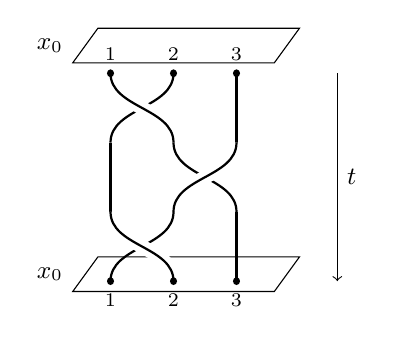
\begin{tikzpicture}[scale=0.8,yscale=1.1]
  % top and bottom planes
  \draw (-0.6,0.15) -- (2.6,0.15) -- (3.0,0.65) -- (-0.2,0.65) -- cycle;
  \draw (-0.6,-3.15) -- (2.6,-3.15) -- (3.0,-2.65) -- (-0.2,-2.65) -- cycle;
  \node[left] at (-0.6,0.4) {\small $x_0$};
  \node[left] at (-0.6,-2.9) {\small $x_0$};
  % level 0: sigma_1 (strand from pos 0 over)
  \draw[thick] (1,0) .. controls (1,-0.5) and (0,-0.5) .. (0,-1);
  \draw[white,line width=5pt] (0,0) .. controls (0,-0.5) and (1,-0.5) .. (1,-1);
  \draw[thick] (0,0) .. controls (0,-0.5) and (1,-0.5) .. (1,-1);
  \draw[thick] (2,0) -- (2,-1);
  % level 1: sigma_2^{-1}
  \draw[thick] (1,-1) .. controls (1,-1.5) and (2,-1.5) .. (2,-2);
  \draw[white,line width=5pt] (2,-1) .. controls (2,-1.5) and (1,-1.5) .. (1,-2);
  \draw[thick] (2,-1) .. controls (2,-1.5) and (1,-1.5) .. (1,-2);
  \draw[thick] (0,-1) -- (0,-2);
  % level 2: sigma_1
  \draw[thick] (1,-2) .. controls (1,-2.5) and (0,-2.5) .. (0,-3);
  \draw[white,line width=5pt] (0,-2) .. controls (0,-2.5) and (1,-2.5) .. (1,-3);
  \draw[thick] (0,-2) .. controls (0,-2.5) and (1,-2.5) .. (1,-3);
  \draw[thick] (2,-2) -- (2,-3);
  \foreach \x/\l in {0/1,1/2,2/3} {
    \fill (\x,0) circle (1.6pt); \node[above] at (\x,0.05) {\scriptsize $\l$};
    \fill (\x,-3) circle (1.6pt); \node[below] at (\x,-3.05) {\scriptsize $\l$};
  }
  \draw[->] (3.6,0) -- (3.6,-3) node[midway,right] {\small $t$};
\end{tikzpicture}
\end{center}
\noindent\textit{Figure:} a loop in $\Conf(3,\R^2)/\Sigma_3$ drawn as a braid on three
strands. \orig{p.\,5: second sketch (strand graphs) illegible, omitted}

\begin{remark}
\added{For $X=\R$ the components of $\Conf(N,\R)$ are contractible
(Example~\ref{L07:ex:confR}), so all braid groups of $\R$ are trivial. For $X=\R^n$ with
$n\geq 3$ the diagonal has codimension $n\geq3$, so $\Conf(N,\R^n)$ is simply connected:
$P_N(\R^n)=1$ and $B_N(\R^n)\cong\Sigma_N$. The plane is the interesting case.}
\end{remark}

\section{Functions on configuration spaces}
\label{L07:sec:functions}

To configurations we would like to associate real-valued functions, based on what they
model. For example:
\begin{itemize}
  \item an electrical potential, or more generally a potential given as a sum of pair
    interactions \added{$E(x_1,\dots,x_N)=\sum_{i<j}\phi(x_i,x_j)$};
  \item a hard shell (hard sphere) potential
    \added{($\phi=+\infty$ if two spheres overlap, $0$ otherwise)};
\end{itemize}
which can describe different energy levels and can also constrain the system.

We may ask about
\begin{itemize}
  \item minima and maxima (local and global);
  \item critical points;
  \item generic configurations.
\end{itemize}
This breaks down into a couple of categories:
\begin{itemize}
  \item small $N$: by hand;
  \item large $N$: by statistical mechanics, or by averaging.
\end{itemize}
The classic example for large $N$ is the expected value of $N$ coin flips with values in
$\{0,1\}$, which leads to the central limit theorem.

\subsection{The Boltzmann distribution}
\label{L07:subsec:boltzmann}

So, for example, consider $N$ particles, each in one of $K$ states, with energy $E_i$
associated to the state $i\in\{1,\dots,K\}$. Let $N_i$ be the number of particles in state
$i$. The system is closed, so the total energy is constant, and
\[
  E=\sum_{i=1}^K E_i N_i, \qquad N=\sum_{i=1}^K N_i .
\]
The number of ways to place the $N$ particles according to the partition
$\{N_1,\dots,N_K\}$ is the multinomial coefficient
\[
  W=\frac{N!}{N_1!\cdots N_K!}.
\]
For large $N$ the optimal partition dominates, so we want to determine the partition that
maximises $W$ \added{subject to the two constraints above}. One can derive the
\emph{Boltzmann measure}
\[
  \frac{N_i}{N}=\frac{e^{-\beta E_i}}{\sum_{j=1}^K e^{-\beta E_j}},
  \qquad\text{i.e.}\qquad
  \Pr(\text{state } i)=\frac{e^{-\beta E_i}}{Z},
\]
where $Z=\sum_{j=1}^K e^{-\beta E_j}$ is the \emph{partition function} and
$\beta=1/(k_B T)$, with $k_B$ \added{Boltzmann's} constant and $T$ the temperature.
\orig{derivation deferred to ``next time'' in the notes}

\begin{addedblock}
Sketch of the derivation. By Stirling's formula,
$\ln W\approx N\ln N-\sum_i N_i\ln N_i$. Maximising this subject to $\sum_i N_i=N$ and
$\sum_i E_iN_i=E$ with Lagrange multipliers $\alpha,\beta$ gives
$-\ln N_i-1-\alpha-\beta E_i=0$, i.e.\ $N_i\propto e^{-\beta E_i}$; normalising gives the
formula above. The multiplier $\beta$ is fixed by the energy constraint, and physics
identifies it with $1/(k_BT)$.
\end{addedblock}

\begin{remark}
Note:
\begin{itemize}
  \item as $T\to\infty$ (so $\beta\to0$), $\Pr(i)\to 1/K$: all states become equally likely;
  \item as $T\to 0$ (so $\beta\to\infty$), $\Pr$ concentrates on the states of minimal
    energy \added{(uniformly on the ground states if there are several)}.
\end{itemize}
\end{remark}

\subsection{A gas in a box}
\label{L07:subsec:gas}

But let us consider another (sketchy) physics analysis: the distribution of a gas in a box,
in the simplest non-interacting setting. Take $2N$ points, i.e.\ a configuration in
\[
  \Conf\big(2N,[-1,1]^3\big),
\]
\added{chosen uniformly at random.} Let $P_m$ be the probability that exactly $N+m$
particles have positive first coordinate.

There are $2^{2N}$ choices for the signs of the first coordinates, all equally likely, and
$\binom{2N}{N+m}$ of them have exactly $N+m$ particles with first coordinate $>0$. (This is
really the coin-flip analysis.) So
\[
  P_m=2^{-2N}\,\frac{(2N)!}{(N+m)!\,(N-m)!}.
\]

We use a very bad version of Stirling's approximation,
\[
  n!\sim\Big(\frac ne\Big)^n\sqrt{2\pi n}\;\leadsto\;n!\approx\Big(\frac ne\Big)^n .
\]
Then
\begin{align*}
  P_m&\approx 2^{-2N}\Big(\frac{2N}{e}\Big)^{2N}\Big/
     \Big[\Big(\frac{N+m}{e}\Big)^{N+m}\Big(\frac{N-m}{e}\Big)^{N-m}\Big]
   =\frac{N^{2N}}{(N+m)^{N+m}(N-m)^{N-m}}\\
  &=\Big(1+\frac mN\Big)^{-(N+m)}\Big(1-\frac mN\Big)^{-(N-m)}
   =\Big(1-\frac{m^2}{N^2}\Big)^{-N}\Big(1+\frac mN\Big)^{-m}\Big(1-\frac mN\Big)^{m}\\
  &\overset{m\ll N}{\approx}\big(e^{-m^2/N^2}\big)^{-N}\big(e^{m/N}\big)^{-m}\big(e^{-m/N}\big)^{m}
   = e^{-m^2/N}.
\end{align*}
Since the crude Stirling formula loses the factors $\sqrt{2\pi n}$, we only keep the shape
and write
\[
  P_m\approx P_0\,e^{-m^2/N}
\]
(a crude central limit theorem). Normalising,
\[
  1=\sum_{m=-N}^{N}P_m\approx\int_{-\infty}^{\infty}P_0\,e^{-m^2/N}\,dm=P_0\sqrt{\pi N}
  \quad\Longrightarrow\quad
  P_0=\frac{1}{\sqrt{\pi N}},\qquad P_m\approx\frac{1}{\sqrt{\pi N}}\,e^{-m^2/N}.
\]
Comparing with $e^{-m^2/(2\sigma^2)}$ we get $\sigma^2=N/2$, so $\sigma=\sqrt{N/2}$.
\added{This agrees with the exact variance $2N\cdot\frac12\cdot\frac12=N/2$ of the
binomial distribution, and $P_0=1/\sqrt{\pi N}$ is exactly what the full Stirling formula
gives for $\binom{2N}{N}4^{-N}$.}

So the number of points with positive first coordinate is approximately Gaussian, centred
at the expected value $N$ with standard deviation $\sqrt{N/2}$. For example, for large $N$,
about $95\%$ of configurations are within $2\sigma=2\sqrt{N/2}$ of the expected value.
\added{The relative fluctuation $\sigma/N=1/\sqrt{2N}$ tends to $0$.}

\begin{remark}
\added{The approximations $\ln(1\pm x)\approx\pm x-x^2/2$ used above each drop cubic
terms of size $m^3/N^2$, but these cancel between the factors $(1+\frac mN)^{-m}$ and
$(1-\frac mN)^{m}$ (the exact exponent is even in $m$). The first neglected term is
$-m^4/(6N^3)$, so the Gaussian approximation is accurate for $m\ll N^{3/4}$; this covers
the typical range $m=O(\sqrt N)$.}\fixed{error order was stated as $m^3/N^2$}
\end{remark}

So if we pick a point in high dimensions, i.e.\ a configuration in
$[-1,1]^{3\cdot 2N}$\fixed{notes: $[-1,1]^{3N}$; $2N$ points in $\R^3$ give $6N$ coordinates}
(and the same argument works for the other variables), we find roughly half of the
coordinates positive and half negative, just like the coin flips. This makes sense.
We can also talk about energy, etc., and generic configurations in this way.

But we may be interested in smaller configurations, like nearest neighbours, where
Stirling's approximation is bad.
\unclear{reading of ``smaller configurations, like nearest neighbours'' uncertain}
How do we analyse such things?

\subsection{Points on the circle}
\label{L07:subsec:circle}

Let us look at points on $\Sph^1$, \added{which we take to have length $1$}. Consider
$\operatorname{Reduced}(3,\Sph^1)$, three points on the circle modulo rotation. Use the
rotation to fix one point at $0$; going around the circle, the three gaps between
consecutive points are $x$, $y$ and $1-x-y$.
\fixed{notes write $1-x+y$}
So the reduced space is described by
\[
  \{(x,y): x>0,\ y>0,\ x+y<1\},
\]
an open triangle, whose boundary edges $x=0$, $y=0$, $x+y=1$ are the collisions.
\added{(For labelled points there are two such triangles, one for each cyclic order of the
labels $1,2,3$; compare Example~\ref{L07:ex:confS1} below.)}
In general, for $N$ points we have a simplex
\added{$\{(g_1,\dots,g_N): g_i>0,\ \sum g_i=1\}$ of gaps, an open $(N-1)$-simplex
(one for each of the $(N-1)!$ cyclic orders of the labels)}.

We can attach the \emph{injectivity radius} function
\[
  \rho=\min_{i\neq j}\tfrac12\,\operatorname{geodesic}(x_i,x_j).
\]
\added{Since the smallest gap is at most $1/N\le 1/2$, $\rho$ is half the smallest gap:
$\rho=\frac12\min(x,y,1-x-y)$ for $N=3$. It has a unique maximum $\rho=1/6$ at the
equilateral configuration $x=y=1/3$; its level sets are triangles, and it fails to be
smooth along the three segments from the centre to the vertices. In general the maximum is
$1/(2N)$, attained at the regular $N$-gon.}

\begin{center}
\begin{tikzpicture}[scale=3.6]
  \draw[dashed] (0,0) -- (1,0) -- (0,1) -- cycle;
  \draw[thin,gray] (1/3,1/3) -- (0,0) (1/3,1/3) -- (1,0) (1/3,1/3) -- (0,1);
  \draw[addcol] (1/6,1/6) -- (2/3,1/6) -- (1/6,2/3) -- cycle;
  \fill (1/3,1/3) circle (0.5pt);
  \draw[gray,thin] (1/3,1/3) -- (0.62,0.62); \node[right] at (0.62,0.64) {\scriptsize $x=y=\tfrac13$};
  \node[below] at (0.5,0) {\scriptsize $y=0$};
  \node[left] at (0,0.5) {\scriptsize $x=0$};
  \node[above right] at (0.72,0.3) {\scriptsize $x+y=1$};
  \node[addcol] at (0.47,0.21) {\tiny $\rho=\frac1{12}$};
\end{tikzpicture}
\end{center}
\noindent\textit{Figure:} $\operatorname{Reduced}(3,\Sph^1)$ as an open triangle
(dashed boundary = collisions), with a level set of $\rho$ and the lines where $\rho$ is
not smooth.

\begin{remark}
\orig{p.\,13: closing remark largely illegible}
\unclear{remark ends ``\dots it's a (box--?)\dots''}
The notes end Lecture~7 with a remark about computing with the injectivity radius.
\added{The point to keep in mind for the next lecture is that $\rho$ is a minimum of smooth
functions, hence only piecewise smooth, so smooth Morse theory does not apply to it
directly.}
\end{remark}

% ======================================================================

\chapter{Lecture 8: (Smooth) Morse theory}
\label{L07:ch:lecture8}

\section{Configuration spaces on a line and Weyl chambers}
\label{L07:sec:weyl}

We started to talk about the spaces
\[
  \Conf(N,X)=\prod_{i=1}^N X\setminus\Delta,
  \qquad
  \Delta=\{(x_i)_{i=1}^N: x_i=x_j \text{ for some } i\neq j\}.
\]

\begin{example}[$\Conf(3,\Sph^1)$]
\label{L07:ex:confS1}
Fixing the first point at $0$ by a rotation, the other two points lie in
$\Sph^1\setminus\{0\}\cong(0,1)$ and must be distinct, so
\[
  \Conf(3,\Sph^1)\cong \Sph^1\times\big((0,1)^2\setminus\{x_2=x_3\}\big),
\]
\added{and the reduced space is the open square minus its diagonal: two open triangles, one
for each cyclic order (cf.\ Section~\ref{L07:subsec:circle}).}
\fixed{notes: ``$\Conf(3,\Sph^1)\approx$ square''; this is the reduced space}
\end{example}

\begin{center}
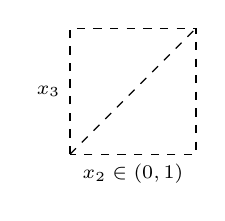
\begin{tikzpicture}[scale=1.6]
  \draw[dashed] (0,0) rectangle (1,1);
  \draw[dashed] (0,0) -- (1,1);
  \node[below] at (0.5,0) {\scriptsize $x_2\in(0,1)$};
  \node[left] at (0,0.5) {\scriptsize $x_3$};
\end{tikzpicture}
\end{center}

\begin{example}[$\Conf(N,\R)$ and the $A_{N-1}$ Weyl chambers]
Write $n=N$. Consider the affine subspaces
\[
  V=V_c=\Big\{(x_i)_{i=1}^n:\ \sum_i x_i=c\Big\}\subset\R^n .
\]
\added{Translation along $(1,\dots,1)$ splits off, $\Conf(n,\R)\cong\R\times(V_c\setminus\Delta)$.}
In these subspaces the hyperplanes $\{x_i=x_j\}\cap V$ are the boundaries of the Weyl
chambers in our construction of the $A_{n-1}$ root system in $V\subset\R^n$.
\added{Recall $A_{n-1}=\{e_i-e_j: i\neq j\}$, with $n(n-1)$ roots, simple roots
$e_i-e_{i+1}$, and Weyl group $\Sigma_n$ generated by the reflections in the hyperplanes
$x_i=x_j$ (i.e.\ swapping two coordinates). The connected components of
$V\setminus\Delta$ are exactly the $n!$ open Weyl chambers.}

For $n=3$\fixed{notes: ``$n=2$''; the example is $A_2$, $n=3$} we had the simple roots
\[
  (1,-1,0),\qquad (0,1,-1).
\]
So the root system is given by the six vectors
\[
  \pm(1,-1,0),\qquad \pm(0,1,-1),\qquad \pm(1,0,-1),
\]
generated by swapping coordinates, i.e.\ by reflecting through the hyperplanes $x_i=x_j$,
$i\neq j$. To draw them in the plane $V_3=\{x+y+z=3\}$ we translate by $(1,1,1)$.
\end{example}

\begin{center}
\begin{tikzpicture}[scale=1.25]
  \coordinate (A) at (-1.732,-1);
  \coordinate (B) at (1.732,-1);
  \coordinate (C) at (0,2);
  \draw (A) -- (B) -- (C) -- cycle;
  \node[below left] at (A) {\scriptsize $(3,0,0)$};
  \node[below right] at (B) {\scriptsize $(0,3,0)$};
  \node[above] at (C) {\scriptsize $(0,0,3)$};
  \coordinate (O) at (barycentric cs:A=1,B=1,C=1);
  % walls (medians)
  \draw[dashed] (C) -- (barycentric cs:A=1,B=1);
  \draw[dashed] (A) -- (barycentric cs:B=1,C=1);
  \draw[dashed] (B) -- (barycentric cs:A=1,C=1);
  \node[below] at (barycentric cs:A=1,B=1) {\scriptsize $x=y$};
  \node[above right] at (barycentric cs:B=1,C=1) {\scriptsize $y=z$};
  \node[above left] at (barycentric cs:A=1,C=1) {\scriptsize $x=z$};
  % roots + (1,1,1)
  \foreach \a/\b/\c in {2/0/1, 0/2/1, 1/2/0, 2/1/0, 1/0/2, 0/1/2} {
    \draw[->,addcol,thick] (O) -- (barycentric cs:A=\a,B=\b,C=\c);
    \fill[addcol] (barycentric cs:A=\a,B=\b,C=\c) circle (1.2pt);
  }
  \fill (O) circle (1.2pt);
  \node[below right] at ($(O)+(0.05,-0.02)$) {\tiny $(1,1,1)$};
  \node[addcol,left] at ($(barycentric cs:A=2,B=0,C=1)+(-0.05,0)$) {\tiny $(2,0,1)$};
\end{tikzpicture}
\end{center}
\noindent\textit{Figure:} the plane $x+y+z=3$. The dashed lines are the walls
$x_i=x_j$; they cut the plane into the six Weyl chambers (the components of
$V_3\setminus\Delta$). The arrows are the six roots of $A_2$, translated by $(1,1,1)$; they
end at the trisection points of the edges, e.g.\ $(1,1,1)+(1,-1,0)=(2,0,1)$, and each
root is perpendicular to one wall.

\subsection{Manifolds}
\label{L07:subsec:manifolds}

We will consider spaces $M$ that are Hausdorff, second countable topological spaces: the
topology separates points, and there is a countable basis for the topology. (Basically
this is to eliminate pathological examples.)

\begin{definition}[Homeomorphism]
A \emph{homeomorphism} $\varphi\colon M\to N$ is a continuous bijection with continuous
inverse. Equivalently: $\varphi$ is a bijection, and $U\subset M$ is open if and only if
$\varphi(U)\subset N$ is open.
\end{definition}

\begin{definition}[Coordinate chart]
A \emph{coordinate chart} for a space $M$ is a homeomorphism from a coordinate
neighbourhood $U$ \added{(an open subset of $M$)} onto an open subset of $\R^n$,
\[
  \varphi_U\colon U\subset M\longrightarrow V\subset\R^n .
\]
\end{definition}

\begin{center}
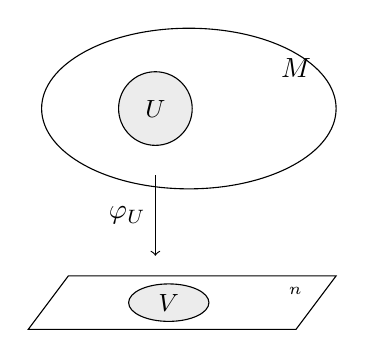
\begin{tikzpicture}[scale=0.85]
  \draw (0,0) ellipse (2.2 and 1.2); \node at (1.6,0.6) {$M$};
  \draw[fill=gray!15] (-0.5,0) circle (0.55); \node at (-0.5,0) {\small $U$};
  \draw[->] (-0.5,-1.0) -- (-0.5,-2.2) node[midway,left] {$\varphi_U$};
  \draw (-2.4,-3.3) -- (1.6,-3.3) -- (2.2,-2.5) -- (-1.8,-2.5) -- cycle;
  \node at (1.6,-2.8) {\small $\R^n$};
  \draw[fill=gray!15] (-0.3,-2.9) ellipse (0.6 and 0.28); \node at (-0.3,-2.9) {\small $V$};
\end{tikzpicture}
\end{center}

A smooth bijection with smooth inverse is a \emph{diffeomorphism}. So in the smooth
setting, coordinate changes should be diffeomorphisms.

A \emph{manifold} is a space $M$ with a collection of charts $\{\varphi_{U_i}\}$ (an
\emph{atlas}), indexed by a cover $\{U_i\}$ of $M$, together with \emph{transition maps}
that patch the charts together:
\[
  \tau_{ij}=\tau_{U_iU_j}=\varphi_{U_j}\circ\varphi_{U_i}^{-1}\colon
  \varphi_{U_i}(U_i\cap U_j)\to\varphi_{U_j}(U_i\cap U_j).
\]

\begin{center}
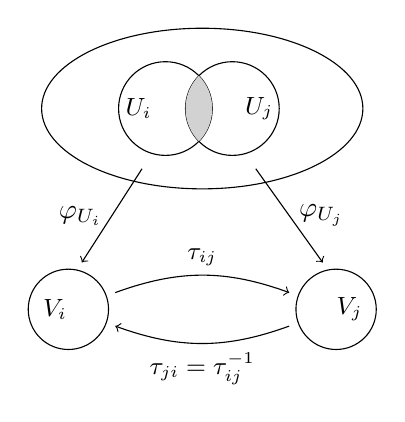
\begin{tikzpicture}[scale=0.85]
  \draw (0,0) ellipse (2.4 and 1.2);
  \draw (-0.55,0) circle (0.7); \draw (0.45,0) circle (0.7);
  \begin{scope} \clip (-0.55,0) circle (0.7); \fill[gray!35] (0.45,0) circle (0.7); \end{scope}
  \node at (-0.95,0) {\small $U_i$}; \node at (0.85,0) {\small $U_j$};
  \draw (-2,-3) circle (0.6); \node at (-2.2,-3) {\small $V_i$};
  \draw (2,-3) circle (0.6); \node at (2.2,-3) {\small $V_j$};
  \draw[->] (-0.9,-0.9) -- (-1.8,-2.3) node[midway,left] {$\varphi_{U_i}$};
  \draw[->] (0.8,-0.9) -- (1.8,-2.3) node[midway,right] {$\varphi_{U_j}$};
  \draw[->] (-1.3,-2.75) to[bend left=20] node[midway,above] {\small $\tau_{ij}$} (1.3,-2.75);
  \draw[->] (1.3,-3.25) to[bend left=20] node[midway,below] {\small $\tau_{ji}=\tau_{ij}^{-1}$} (-1.3,-3.25);
\end{tikzpicture}
\end{center}

\begin{definition}[Smooth structure]
\label{L07:def:smoothstructure}
A \emph{smooth differentiable structure} on $M$ is a collection of (smooth) coordinate
charts $\varphi_i\colon U_i\to V_i\subset\R^n$, $U_i\subset M$, such that
\begin{enumerate}
  \item $M=\bigcup_i U_i$;
  \item every transition map $\tau_{ij}=\varphi_j\circ\varphi_i^{-1}$ is smooth
    \added{(on its domain $\varphi_i(U_i\cap U_j)$)};
  \item it is a \emph{maximal} atlas: if a chart is compatible with all $\varphi_i$ as
    above, then it is in the collection.
\end{enumerate}
A topological space with a smooth structure is a \emph{smooth manifold} (of dimension $n$).
\end{definition}

Basically we can ignore maximality for computations, as maximal atlases are ``unique'':
\added{every atlas satisfying (1) and (2) is contained in exactly one maximal atlas, so it
suffices to write down any atlas.}

\section{Examples; smooth maps}
\label{L07:sec:examples}

\begin{example}
\label{L07:ex:manifolds}
\leavevmode
\begin{itemize}
  \item $\R^n$: choose the identity map as the chart \added{(one chart, $U=\R^n$)}.
  \item $\C^n\to\R^{2n}$, using $(\operatorname{Re},\operatorname{Im})$ on each $U_i$.
  \item $\Sph^n\to\R^n$: stereographic projection on $\Sph^n\setminus\{N\}$ and on
    $\Sph^n\setminus\{S\}$ \added{(north and south poles; the transition map is the
    inversion $y\mapsto y/\abs{y}^2$ on $\R^n\setminus\{0\}$, which is smooth)}.
  \item On tori, by products of the $\Sph^1$ charts.
  \item On open subsets of manifolds, by carrying over the subspace topology
    \added{and restricting the charts}.
\end{itemize}
\added{In particular $\Conf(N,X)$ is an open subset of $X^N$, so it is a smooth manifold of
dimension $N\dim X$ whenever $X$ is.}
\end{example}

We can define \emph{smooth maps} between manifolds.

\begin{definition}[Smooth map]
\label{L07:def:smoothmap}
A map $f\colon M\to N$ is \emph{smooth} if for each $p\in M$ and some charts $\varphi$ on
$U\ni p$ for $M$ and $\psi$ on $V\ni f(p)$ for $N$ (and then for all such charts),
\added{with $f(U)\subset V$,} the induced map
\[
  \begin{array}{ccc}
    U & \xrightarrow{\ f\ } & V\\[2pt]
    {\scriptstyle\varphi}\downarrow & & \downarrow{\scriptstyle\psi}\\[2pt]
    \varphi(U) & \xrightarrow{\ \psi f\varphi^{-1}\ } & \psi(V)
  \end{array}
\]
$\psi\circ f\circ\varphi^{-1}$ is smooth on its domain.
\added{(``Some $\Rightarrow$ all'' because the transition maps are smooth.)}
\end{definition}
\orig{p.\,12 (= scan p.\,25) repeats this diagram}

Similarly for maps between manifolds of other kinds. So we can define diffeomorphisms
(homeomorphisms) of manifolds: a (smooth) bijection $M\to N$ with (smooth) inverse,
written $M\cong N$.
If we change the underlying conditions on the maps \added{(e.g.\ continuous, $C^k$, or
piecewise linear transition maps)} we can still define coordinate charts, atlases, etc.
\orig{crossed out: ``Sadly, not all the maps we want to work with will be smooth''}

\section{Homotopy type}
\label{L07:sec:homotopy}

\orig{a first ``8.3 Morse theory'' is crossed out here}
We will want to talk about \emph{homotopy type} as well, since we may be dealing with
things that are not diffeomorphic but are topologically ``similar''.

\begin{definition}[Homotopy]
\label{L07:def:homotopy}
Two maps $f,g\colon M\to N$ are \emph{homotopic}, written $f\simeq g$, if there exists a
continuous function
\[
  H\colon M\times I\to N,\qquad I=[0,1],
\]
such that $H(x,0)=f(x)$ and $H(x,1)=g(x)$ for all $x\in M$.
\end{definition}

\begin{definition}[Homotopy equivalence]
\label{L07:def:hequiv}
Two (smooth) spaces $M$ and $N$ are \emph{homotopy equivalent} (have the same homotopy
type) if there are maps
\[
  f\colon M\to N,\qquad g\colon N\to M
  \qquad\text{such that}\qquad
  f\circ g\simeq\mathrm{id}_N,\quad g\circ f\simeq\mathrm{id}_M .
\]
\orig{letters $X,Y$ corrected to $M,N$ in blue on the page}
\end{definition}

The idea: the spaces can be continuously (smoothly) deformed into each other.

\begin{example}[$D^2\simeq\{0\}$]
\label{L07:ex:disk}
Let $f\colon D^2\to\{0\}$ be the radial retraction to $0$ (the constant map) and
$g\colon\{0\}\to D^2$ the inclusion. In polar coordinates put
\[
  h\big(t,(r,\theta)\big):=\big((1-t)r,\theta\big).
\]
Then $h(0,\cdot)=\mathrm{id}_{D^2}$ and $h(1,\cdot)=g\circ f$ (the map $D^2\to 0$), so
$g\circ f\simeq\mathrm{id}_{D^2}$; and $f\circ g=\mathrm{id}_{\{0\}}$.
\added{($h$ is continuous also at $r=0$, since $(1-t)\cdot 0=0$ regardless of $\theta$.)}
\end{example}

\begin{definition}[Relative homotopy; deformation retract]
\label{L07:def:relhom}
A \emph{homotopy relative to a subspace} is a homotopy which fixes the points of the
subspace: for $f,g\colon M\to N$ and $K\subset M$, $f$ and $g$ are \emph{homotopic
relative to $K$} if there is a homotopy $h\colon M\times I\to N$ between $f$ and $g$ such
that
\[
  h(k,t)=f(k)=g(k)\qquad\text{for all } k\in K,\ t\in I .
\]
If $f=\mathrm{id}_M$ and $g$ is a \emph{retraction}, i.e.\ a continuous map $M\to K$ with
$g|_K=\mathrm{id}$ \added{(followed by the inclusion $K\hookrightarrow M$)}, then this
homotopy defines a \emph{strong deformation retraction} of $M$ onto $K$.
\end{definition}
See the last example: $h$ is a strong deformation retraction of $D^2$ onto $\{0\}$.

\section{An aside about homotopy groups}
\label{L07:sec:homotopygroups}

We consider homotopy classes of maps to pointed spaces
\added{(with homotopies relative to the base point)}. Consider
$f\colon \Sph^1\to(X,x_0)$, or equivalently paths $f\colon I\to X$ with
$f(0)=f(1)=x_0$. These have a group structure under concatenation,
\[
  (f\cdot g)(t)=\begin{cases} f(2t), & t\in[0,\tfrac12],\\ g(2t-1), & t\in[\tfrac12,1].\end{cases}
\]
This is the fundamental group $\pi_1(X,x_0)$.

In general one can consider maps $f\colon\Sph^n\to(X,x_0)$, viewed as maps
$f\colon I^n\to X$ with $f(\partial I^n)=x_0$, with concatenation defined appropriately
\added{(in the first coordinate)}; this gives $\pi_n(X,x_0)$. If $X$ is path connected we
may ignore the base point $x_0$ \added{(up to isomorphism)}.

\begin{example}
Draw $(D^2,x_0)\setminus\{0\}$.
\orig{example left blank on the page}
\added{The punctured disk deformation retracts (radially) onto the circle of radius
$\abs{x_0}$, so $\pi_1(D^2\setminus\{0\},x_0)\cong\pi_1(\Sph^1)\cong\Z$, generated by
the loop going once around the puncture. Compare $\pi_1(D^2)=0$ from
Example~\ref{L07:ex:disk}: removing a point changes the homotopy type.}
\end{example}

We will not deal with this too much, but note that this is a nice invariant for spaces:
\added{homotopy equivalent spaces have isomorphic homotopy groups.} This is also the
source of the braid groups of Section~\ref{L07:sec:braid}.

\section{Morse theory}
\label{L07:sec:morse}
\orig{numbered ``8.2'' in the notes}

Morse theory is a fairly general way to study manifolds and functions on them. The idea is
that the structure of the sets of critical points of functions and the topological
structure of the manifold are related. (We will follow Milnor and others
\added{(see J.~Milnor, \emph{Morse Theory}, Annals of Math.\ Studies 51, Part~I)}.)

\begin{example}[The classic picture]
\label{L07:ex:torus}
Consider $f\colon\T^2\to\R$ given by
\[
  \T^2\hookrightarrow\R^3\xrightarrow{\ \mathrm{proj}_z\ }\R,
\]
the height function $h=\mathrm{proj}_z(x,y,z)=z$ on a torus standing upright, normalised
so that it takes values in $[0,1]$. It has four critical points: $p$ (minimum, height $0$),
$q$ and $r$ (the bottom and top of the hole) and $s$ (maximum, height $1$).
\end{example}

\begin{center}
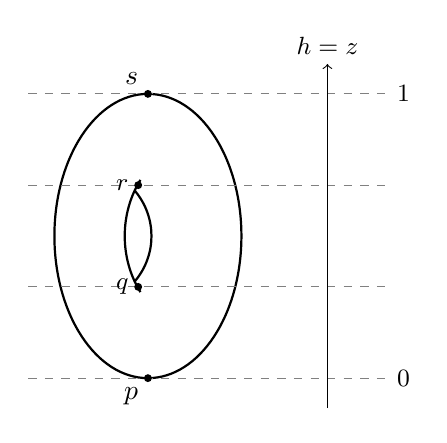
\begin{tikzpicture}[scale=0.95]
  \draw[thick] (0,0) ellipse (1.25 and 1.9);
  \draw[thick] (-0.1,-0.75) .. controls (-0.38,-0.3) and (-0.38,0.3) .. (-0.1,0.75);
  \draw[thick] (-0.17,-0.6) .. controls (0.12,-0.25) and (0.12,0.25) .. (-0.17,0.6);
  \foreach \y/\n in {-1.9/p,-0.68/q,0.68/r,1.9/s} {
    \draw[dashed,gray] (-1.6,\y) -- (3.2,\y);
  }
  \fill (0,-1.9) circle (1.5pt) node[below left] {$p$};
  \fill (-0.13,-0.68) circle (1.5pt) node[left] {\small $q$};
  \fill (-0.13,0.68) circle (1.5pt) node[left] {\small $r$};
  \fill (0,1.9) circle (1.5pt) node[above left] {$s$};
  \node[right] at (3.2,-1.9) {\small $0$};
  \node[right] at (3.2,1.9) {\small $1$};
  \draw[->] (2.4,-2.3) -- (2.4,2.3) node[above] {\small $h=z$};
\end{tikzpicture}
\end{center}
\noindent\textit{Figure:} the torus standing on the plane $z=0$, seen from the side, with
the height function and its critical points.

Consider the \emph{sublevel sets}
\[
  M_a:=\{x\in M: f(x)<a\}.
\]
\added{(Milnor uses $M^a=\{f\le a\}$; for $a$ not a critical value the two have the same
homotopy type.)}
\begin{itemize}
  \item $a<0=f(p)$: $M_a=\emptyset$.
  \item $f(p)<a<f(q)$: $M_a$ is a $2$-cell, i.e.\ a $2$-ball (a disk).
  \item $f(q)<a<f(r)$: $M_a$ is a cylinder.
  \item $f(r)<a<f(s)$: $M_a$ is a torus minus a disk.
  \item $f(s)<a$: $M_a$ is the whole torus.
\end{itemize}

Up to homotopy, these are handle or \emph{cell attachments}.

\begin{definition}[Attaching a cell]
\label{L07:def:cell}
Let $e^k$ be a closed $k$-dimensional ball, with $\partial e^k=\Sph^{k-1}$, let $Y$ be a
topological space and $g\colon\Sph^{k-1}\to Y$ continuous. Then $Y\cup_g e^k$, the result
of \emph{attaching a $k$-cell to $Y$ by $g$}, is defined as
\[
  Y\cup_g e^k=\big(Y\sqcup e^k\big)/\sim,
  \qquad x\sim g(x)\ \text{ for } x\in\Sph^{k-1}.
\]
\end{definition}

\orig{scan pp.\,28--29 are in reverse order (circled 16, 15)}
The sublevel sets of the torus, up to homotopy, are:
\begin{itemize}
  \item a disk $\simeq$ a point ($0$-cell);
  \item the cylinder $\simeq$ a disk with a $1$-handle attached (a ``U'' shape)
    $\simeq$ a point with a $1$-cell attached, i.e.\ a circle;
  \item the torus minus a disk $\simeq$ a disk with two $1$-handles
    $\simeq$ a point with two $1$-cells attached, i.e.\ a figure eight
    $\Sph^1\vee\Sph^1$;
  \item the torus $\simeq$ the figure eight with a $2$-cell attached
    \added{along the loop $aba^{-1}b^{-1}$}.
\end{itemize}
\orig{p.\,15: sketches of the handle pictures; one equivalence marked ``?''}

\begin{center}
\begin{tikzpicture}[scale=0.85]
  % point
  \fill (0,0) circle (2pt);
  \node at (0,-1.3) {\small $\{p\}$};
  % circle
  \begin{scope}[xshift=2.4cm]
    \draw[thick] (0,0.5) circle (0.5); \fill (0,0) circle (2pt);
    \node at (0,-1.3) {\small $e^0\cup e^1$};
  \end{scope}
  % figure eight
  \begin{scope}[xshift=5.2cm]
    \draw[thick] (-0.5,0) circle (0.5); \draw[thick] (0.5,0) circle (0.5);
    \fill (0,0) circle (2pt);
    \node at (0,-1.3) {\small $e^0\cup e^1\cup e^1$};
  \end{scope}
  % torus as square
  \begin{scope}[xshift=8.4cm,yshift=-0.6cm]
    \fill[gray!15] (0,0) rectangle (1.2,1.2);
    \draw[thick,->] (0,0) -- (0.65,0); \draw[thick] (0.6,0) -- (1.2,0);
    \draw[thick,->] (0,1.2) -- (0.65,1.2); \draw[thick] (0.6,1.2) -- (1.2,1.2);
    \draw[thick,->] (0,0) -- (0,0.65); \draw[thick] (0,0.6) -- (0,1.2);
    \draw[thick,->] (1.2,0) -- (1.2,0.65); \draw[thick] (1.2,0.6) -- (1.2,1.2);
    \node[below] at (0.6,0) {\scriptsize $a$}; \node[above] at (0.6,1.2) {\scriptsize $a$};
    \node[left] at (0,0.6) {\scriptsize $b$}; \node[right] at (1.2,0.6) {\scriptsize $b$};
    \node at (0.6,-0.7) {\small $\cdots\cup e^2=\T^2$};
  \end{scope}
  \node at (1.2,0) {$\leadsto$};
  \node at (3.75,0) {$\leadsto$};
  \node at (7.0,0) {$\leadsto$};
\end{tikzpicture}
\end{center}
\noindent\textit{Figure:} homotopy types of the sublevel sets $M_a$ as $a$ passes
$p$, $q$, $r$, $s$.

The homotopy type (and the diffeomorphism type, outside of a neighbourhood) changes
exactly at the critical points of the function $f$: those points where the gradient is
zero, $\nabla f=0$.

If we look at the Hessian \added{$\Hess f_x=\big(\partial^2 f/\partial u_i\partial u_j(x)\big)$
in local coordinates $u$}, which here is non-degenerate at each critical point, we see
\added{(writing the signature as (\#positive, \#negative) eigenvalues)}:
\[
  \operatorname{sig}(\Hess f_p)=(2,0),\qquad
  \operatorname{sig}(\Hess f_q)=\operatorname{sig}(\Hess f_r)=(1,1),\qquad
  \operatorname{sig}(\Hess f_s)=(0,2).
\]
We call the negative part the \emph{index}, i.e.\ the number of decreasing directions at the
critical point, and we see that it corresponds to the dimension of the attached cell:
index $0$ at $p$ ($0$-cell), index $1$ at $q$ and $r$ ($1$-cells), index $2$ at $s$
($2$-cell).

This is why we want to start with smooth functions.

\begin{definition}[Morse function]
\label{L07:def:morse}
We will call a smooth function $f\colon M\to\R$ \emph{Morse} if it has no degenerate
critical points\fixed{notes say ``no nondegenerate critical pts''}, i.e.\ \added{at every
critical point $x$ (where $df_x=0$) the Hessian $\Hess f_x$ is a non-singular matrix}.
\end{definition}

We will formalise this next time.

\begin{addedblock}
For reference, the two basic theorems (Milnor, \emph{Morse Theory}, Thms.~3.1 and 3.2):
let $f\colon M\to\R$ be smooth and write $M^a=f^{-1}(-\infty,a]$.
(A) If $a<b$, $f^{-1}[a,b]$ is compact and contains no critical points, then $M^a$ is
diffeomorphic to $M^b$, and $M^a$ is a deformation retract of $M^b$.
(B) If $x$ is a non-degenerate critical point of index $\lambda$ with $f(x)=c$, and
$f^{-1}[c-\varepsilon,c+\varepsilon]$ is compact and contains no other critical point, then
for small $\varepsilon>0$, $M^{c+\varepsilon}$ has the homotopy type of
$M^{c-\varepsilon}\cup e^{\lambda}$.
\end{addedblock}
